Wie tief ist der See? (s. Abbildung \ref{ex-trigonometry-1-img-a})
\noindent
"Nehmen wir an, die Wasserlilie ragte, wie in unserer Zeichnung, 10 Zoll über die Oberfläche hinaus und verschwände darunter, wenn man sie zur Seite ziehen würde, 21 Zoll von ihrem ursprünglichen Standort entfernt. Wie tief ist dann das Wasser?" (Mathematische Rätsel und Spiele, Der Klassiker, Sam Loyd, Martin Gardner)

\end{enumerate}

\begin{figure}[ht]
	\centering
	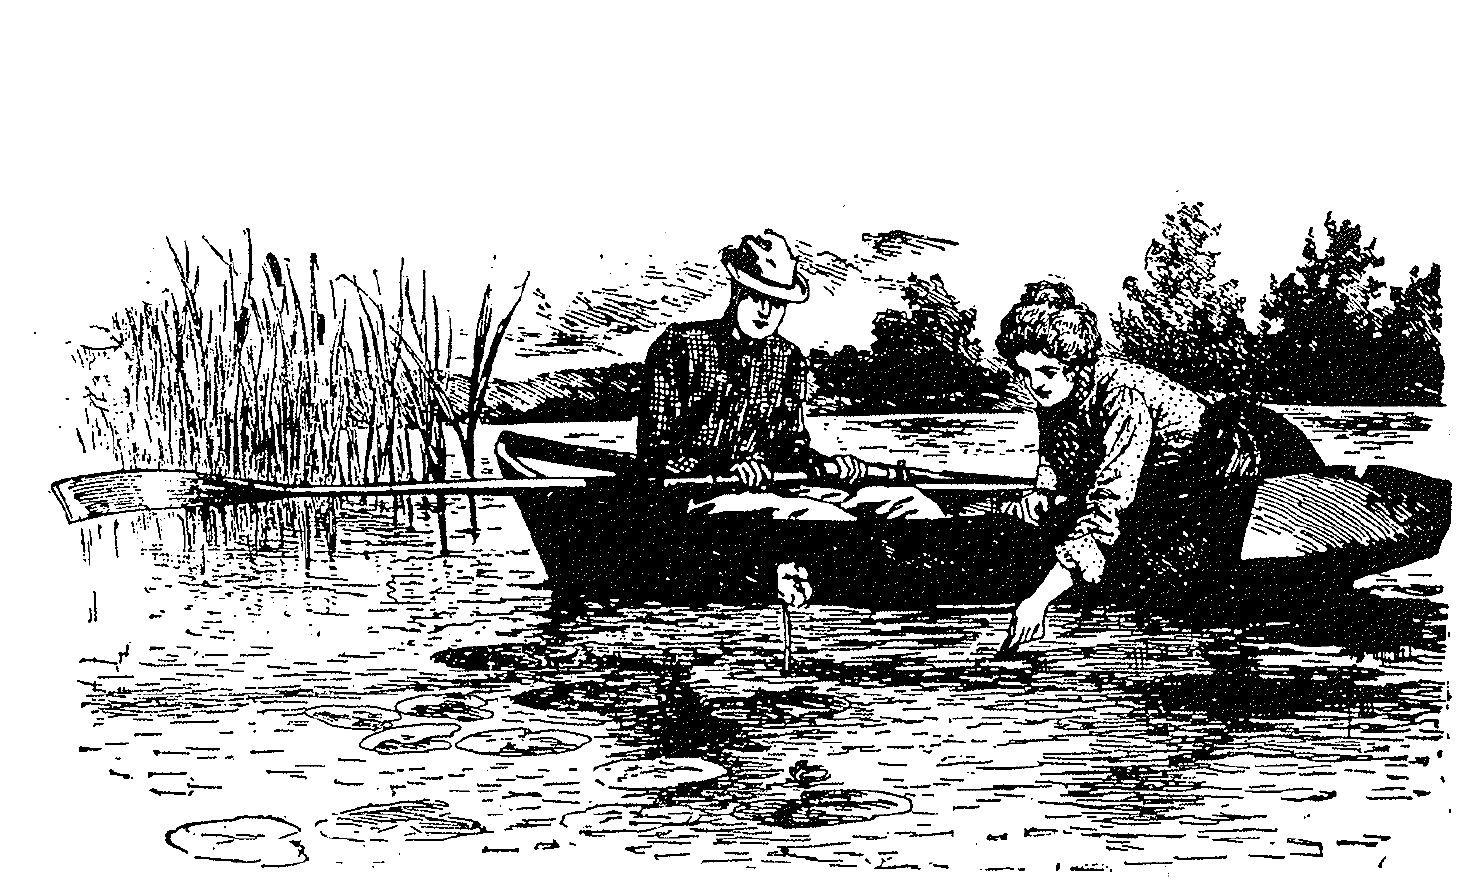
\includegraphics[width=0.45\textwidth]{../pool/ex-trigonometry-1-img-a.png}
	\caption{Skizze zur Rätselaufgabe über die Wasserlilie}.
	\label{ex-trigonometry-1-img-a}
\end{figure}

